% Figure 2 — results (fixed bar labels and spacing)
\begin{figure}[t]
\centering
\begin{subfigure}[t]{0.63\linewidth}
\centering
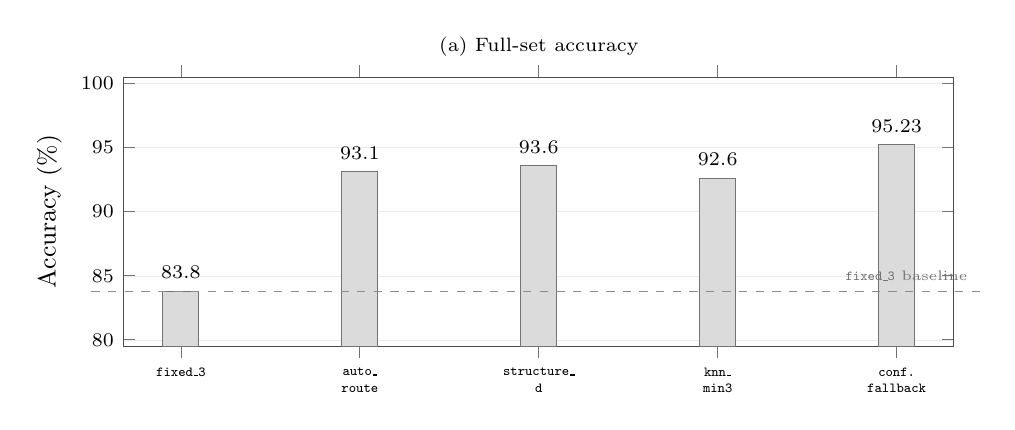
\begin{tikzpicture}
\begin{axis}[
  width=\linewidth,
  height=5.0cm,
  ybar,
  bar width=13pt,
  enlarge x limits=0.08,
  ymin=79.5,
  ymax=100.5,
  ytick={80,85,90,95,100},
  ylabel={Accuracy (\%)},
  xtick={1,2,3,4,5},
  xticklabels={%
    {\texttt{fixed\_3}},
    {\texttt{auto\_\\route}},
    {\texttt{structure\_\\d}},
    {\texttt{knn\_\\min3}},
    {\texttt{conf.\\fallback}}%
  },
  xticklabel style={font=\tiny, align=center, text width=1.15cm},
  ylabel style={font=\small},
  tick label style={font=\scriptsize},
  axis line style={black!70, line width=0.35pt},
  tick style={black!55, line width=0.3pt},
  ymajorgrids=true,
  grid style={black!8, line width=0.2pt},
  title={\scriptsize (a) Full-set accuracy},
  title style={at={(0.5,1)}, yshift=-2pt},
  clip=false
]
\addplot[
  fill=black!14, draw=black!55, line width=0.35pt,
  nodes near coords={\pgfmathprintnumber[fixed,precision=2]{\pgfplotspointmeta}},
  every node near coord/.append style={font=\scriptsize, yshift=1pt}
] coordinates {(1,83.8) (2,93.1) (3,93.6) (4,92.6) (5,95.23)};
\draw[black!45, line width=0.4pt, dashed] (axis cs:0.5,83.8) -- (axis cs:5.5,83.8);
\node[anchor=south east, font=\tiny, text=black!55] at (axis cs:5.45,83.85)
  {\texttt{fixed\_3} baseline};
\end{axis}
\end{tikzpicture}
\caption*{}
\label{fig:bar-a}
\end{subfigure}
\hfill
\begin{subfigure}[t]{0.34\linewidth}
\centering
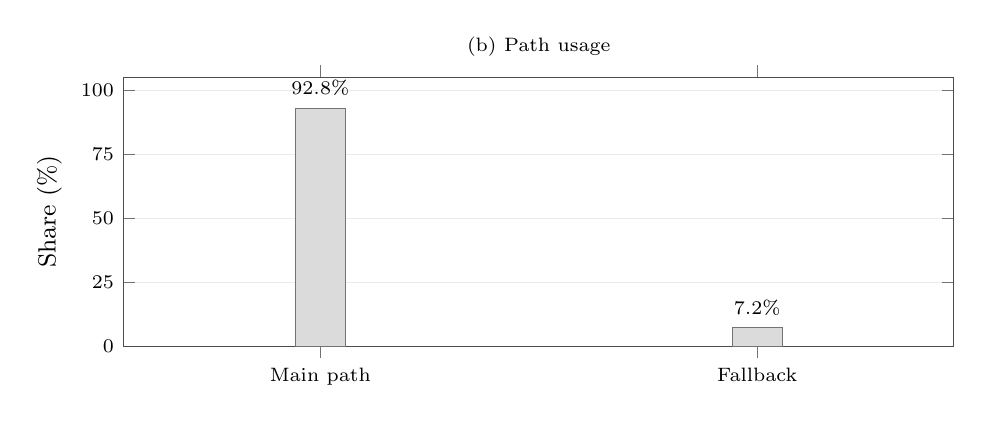
\begin{tikzpicture}
\begin{axis}[
  width=\linewidth,
  height=5.0cm,
  ybar,
  bar width=18pt,
  enlarge x limits=0.45,
  ymin=0,
  ymax=105,
  ytick={0,25,50,75,100},
  ylabel={Share (\%)},
  xtick={1,2},
  xticklabels={{Main path},{Fallback}},
  xticklabel style={font=\scriptsize, align=center},
  ylabel style={font=\small},
  tick label style={font=\scriptsize},
  axis line style={black!70, line width=0.35pt},
  tick style={black!55, line width=0.3pt},
  ymajorgrids=true,
  grid style={black!8, line width=0.2pt},
  title={\scriptsize (b) Path usage},
  title style={at={(0.5,1)}, yshift=-2pt},
  clip=false
]
\addplot[
  fill=black!14, draw=black!55, line width=0.35pt,
  nodes near coords={\pgfmathprintnumber[fixed,precision=1]{\pgfplotspointmeta}\%},
  every node near coord/.append style={font=\scriptsize, yshift=1pt}
] coordinates {(1,92.8) (2,7.2)};
\end{axis}
\end{tikzpicture}
\caption*{}
\label{fig:bar-b}
\end{subfigure}
\caption{Comparison on ProsQA (419 questions). \textbf{(a)} Answer accuracy across five methods; dashed line: \texttt{fixed\_3} (83.8\%). \textbf{(b)} Share of instances using the main path versus fallback ($\tau=0.48$).}
\label{fig:bar}
\end{figure}
